\documentclass{article}

\usepackage{amsmath}
\usepackage{amssymb}
\usepackage{graphicx}
\usepackage{tikz}
\usetikzlibrary{arrows}
\usepackage{verbatim}
%\usepackage{sfmath}
\usepackage{psfrag}
\usepackage{here} 
\usepackage{hyperref}
\usepackage{xcolor}
\usepackage{tcolorbox}


%\textheight=24cm

%\renewcommand\sfdefault{phv}     %use helvetica for sans serif
\renewcommand{\familydefault}{\sfdefault}
\renewcommand{\familydefault}{cmss}

\begin{document}

\section*{Pr\'actica 1. Dynamic model of a robot manipulator with the Lagrange method.}

Consider the robot manipulator represented in Figure~\ref{fig:figure_1}, which moves in a vertical plane.


\begin{figure}[H]
\centerline{\hspace{0cm}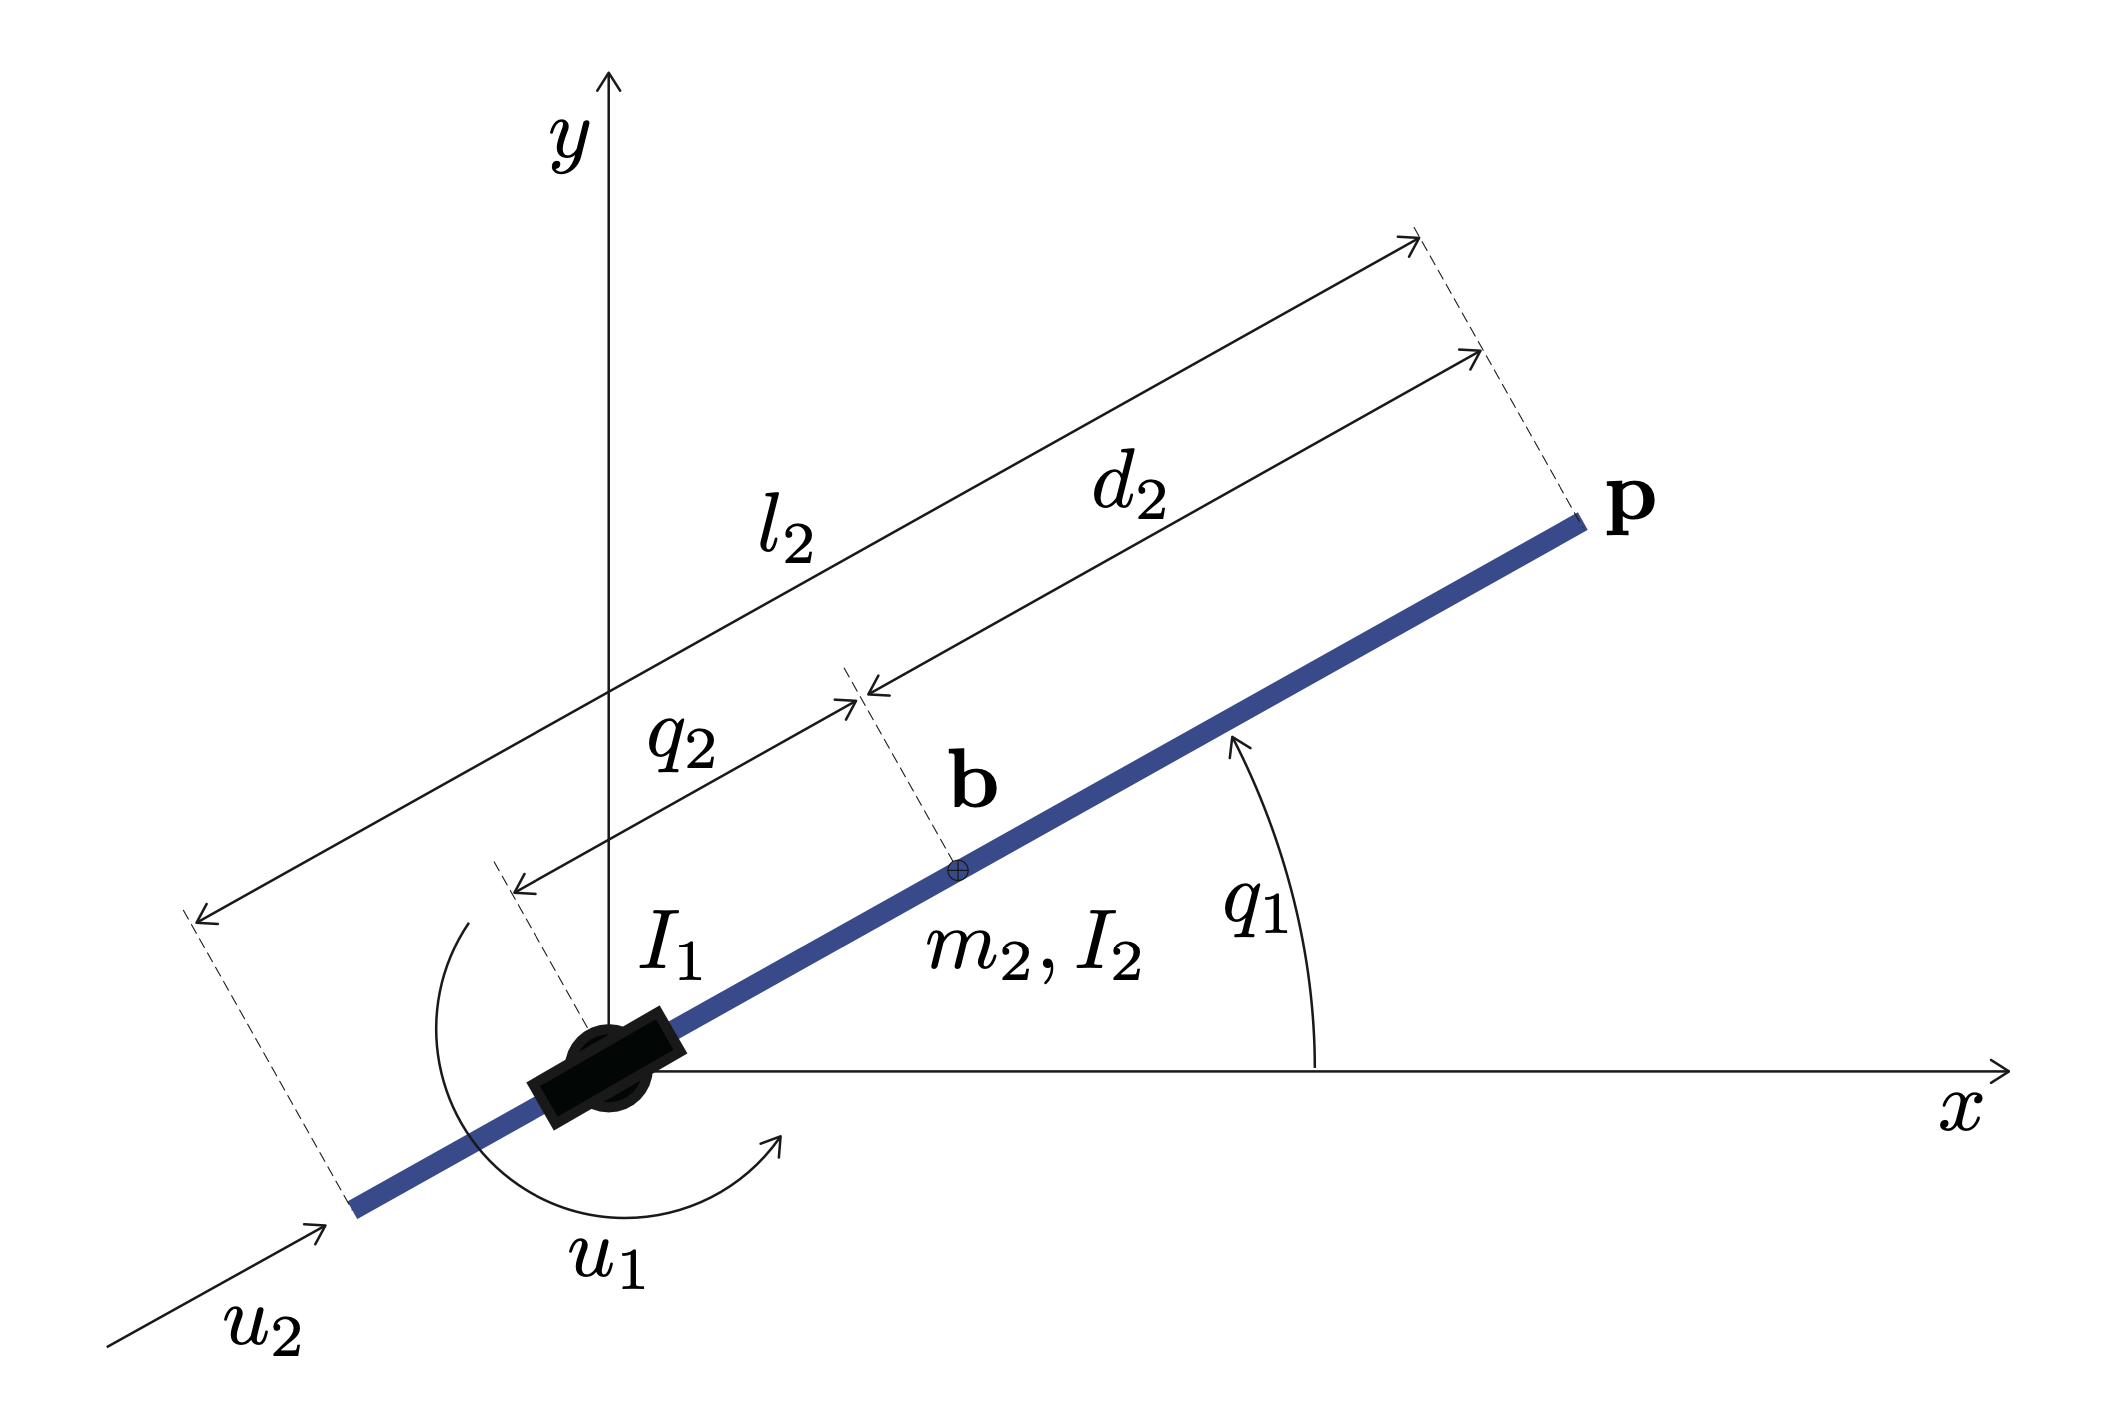
\includegraphics[width=0.66\columnwidth]{drawing}}
\caption{Planar robot manipulator that moves in a vertical plane.}
\label{fig:figure_1}
\end{figure}


The dynamic model of this robotic system is represented by the
second order differential equation 
\begin{equation*}
\mathbf{B}(\mathbf{q}) \ddot{\mathbf{q}}+ \mathbf{C}(\mathbf{q}, \dot{\mathbf{q}}) + \mathbf{N}(\mathbf{q}) = \mathbf{u},
%\label{eq:dynamic_model}
\end{equation*}
where the two matrices $\mathbf{B}(\mathbf{q})$ and $\mathbf{C}(\mathbf{q}, \dot{\mathbf{q}})$ have the following expressions
\begin{eqnarray*}
\mathbf{B}(\mathbf{q}) &=&
\begin{bmatrix}
I_1 + I_2 + m_2 q_2^2 &0\\
0 & m_2
\end{bmatrix},\\
\mathbf{C}(\mathbf{q}, \dot{\mathbf{q}}) 
&=& 
\begin{bmatrix} 
2 m_2 q_2 \dot{q}_1  \dot{q}_2\\
- m_2 q_2 \dot{q}_1^2
\end{bmatrix},\\
\mathbf{N}(\mathbf{q}) 
&=& 
m_2 g
\begin{bmatrix}
q_2 \cos q_1\\
\sin q_1 
\end{bmatrix}.
\end{eqnarray*}

$
\mathbf{q} =
(
q_1, q_2
)^T
$ 
is the vector of configuration variables, where $q_1$ is the
angular position of the link with respect to the $x$ axis of the reference
frame $\{x, y\}$ and $q_2$ is the linear position of the center of mass $\mathbf{b}$ of the link with respect to the origin of the reference frame.
The
vector
$
\dot{\mathbf{q}} =
(\dot{q}_1,
\dot{q}_2)^T
$ 
is the vector of joint velocities, where $\dot{q}_1$ is an angular
velocity and $\dot{q}_2$ is a linear velovity. The vector
$
\ddot{\mathbf{q}} =
(\ddot{q}_1,
\ddot{q}_2)^T
$
is the vector of accelerations, where  $\ddot{q}_1$ is an angular
acceleration and $\ddot{q}_2$ is a linear acceleration. The control inputs of the system are
$
\mathbf{u} =
(u_1,
u_2)^T
$,
where $u_1$ is the torque applied by the angular actuator to the link and
$u_2$ is the force applied by the linear actuator to the link. 
$I_1$ is the barycentric moment of inertia of the angular and linear actuators,
$I_2$ is the barycentric moment of inertia of the link, and $m_2$ is the mass of the link.








\begin{itemize}
\item[a.] Demonstrate the equations of the dynamic model using the Lagrange method.


\item[b.] 
Compute the state space representation of the dynamics of the manipulator in which $\mathbf{x} = (x_1,x_2,x_3,x_4)^T= (q_1, q_2, \dot{q}_1, \dot{q}_2)^T$. Take the coordinates of point $\mathbf{p}$ as the output variables.


\end{itemize}



\noindent
\textcolor{red}{Write a detailed report answering each question in a different section. 
Originality and completeness of the answers will be the aspects that will be taken into account in the grading of the report. 
} 

\newpage













\section*{Solution of Práctica 1}


\begin{itemize}

\item[a.] 
\textcolor{gray}{Demonstrate the equations of the dynamic model using the Lagrange method.}

\bigskip

Mediante el metodo de Lagrange hallamos las ecuaciones de estado del modelo dinamico, sabiendo que: L = T - V\\

La energía cinética T se descompone en la suma de la energía cinética angular y lineal:\\\\
$T_{ang} = \frac{1}{2}(I_1 + I_2)\dot{q_1}^2$,\\\\

$T_{lin} = \frac{1}{2}m_2\dot{q_1}^2q_2^2 + \frac{1}{2}m_2\dot{q_2}^2$\\

La energía potencial es $V = m_2gh$, siendo $h = q_2_y = sen(q_1)q_2$.

Por tanto,\\

$L = \frac{1}{2}(I_1 + I_2 + m_2q_2^2)\dot{q_1}^2 + \frac{1}{2}m_2\dot{q_2}^2 - m_2gsen(q_1)q_2$\\

De este modo, obtenemos las dos siguientes ecuaciones de Lagrange,\\
la primera:\\

		$\frac{\partial L}{\partial \dot{q_1}} = (I_1 + I_2)\dot{q_1} + m_2q_2^2\dot{q_1}$\\\\
		$\frac{d}{dt}\frac{\partial L}{\partial \dot{q_1}} = (I_1 + I_2 + m_2q_2^2)\ddot{q_1} + 2mq_1\dot{q_1}\dot{q_2}$\\\\
		$\frac{\partial L}{\partial q_1} = -m_2gcos(q_1)q_2$\\\\
		
		$(I_1 + I_2 + m_2q_2^2)\ddot{q_1} + 2mq_2\dot{q_1}\dot{q_2} + m_2gcos(q_1)q_2 = u_1$\\
		
y la segunda:\\\\
		$\frac{\partial L}{\partial \dot{q_2}} = m_2\dot{q_2}$\\\\
		$\frac{d}{dt}\frac{\partial L}{\partial \dot{q_2}} = m_2\ddot{q_2}$\\\\
		$\frac{\partial L}{\partial q_2} = m_2q_2\dot{q_1}^2 - m_2gsen(q_1)$\\\\
		
		$m_2\ddot{q_2} - m_2q_2\dot{q_1}^2 + m_2gsen(q_1) = u_2$\\
		

Por lo tanto, escribiendo las ecuaciones en forma matricial obtenemos:\\

$\begin{bmatrix}
I_1 + I_2 + m_2 q_2^2 &0\\
0 & m_2
\end{bmatrix}\ddot{q}
 + 
\begin{bmatrix} 
2 m_2 q_2 \dot{q}_1  \dot{q}_2\\
- m_2 q_2 \dot{q}_1^2
\end{bmatrix}
 + 
\begin{bmatrix}
m_2gcos(q_1)q_2\\
m_2gsen(q_1)
\end{bmatrix}
 = u
$

Finalmente,

	$\ddot{q} = \begin{pmatrix}
	\frac{2\dot{q_1}\dot{q_2}m_2q_2 - u_1 + gm_2q_2cos(q_1))}{m_2q_2^2 + I_1 + I_2}\\
	\frac{m_2q_2\dot{q_1}^2 + u_2 - gm_2sin(q_1)}{m_2}
	\end{pmatrix}
	$
		


\item[b.]
\textcolor{gray}{Compute the state space representation of the dynamics of the manipulator in which $\mathbf{x} = (x_1,x_2,x_3,x_4)^T= (q_1, q_2, \dot{q}_1, \dot{q}_2)^T$. Take the coordinates of point $\mathbf{p}$ as the output variables.}

Asumiendo que:\\\\
		$x = 
			\begin{pmatrix}
				 x_1\\x_2\\x_3\\x_4
			\end{pmatrix}
		 		= 
			\begin{pmatrix}
				 q_1\\q_2\\\dot{q_1}\\\dot{q_2}
			\end{pmatrix}$,\\\\
podemos escribir:\\\\
		$\frac{d}{dt}
			\begin{pmatrix}
				 q_1\\q_2\\\dot{q_1}\\\dot{q_2}
			\end{pmatrix}
				=
			\begin{pmatrix}
				 \dot{q_1}\\\dot{q_2}\\\ddot{q_1}\\\ddot{q_2}
			\end{pmatrix}
				=
			\begin{pmatrix}
				 \dot{q_1}\\\dot{q_2}\\\frac{2\dot{q_1}\dot{q_2}m_2q_2 - u_1 + gm_2q_2cos(q_1))}{m_2q_2^2 + I_1 + I_2}\\\frac{m_2q_2\dot{q_1}^2 + u_2 - gm_2sin(q_1)}{m_2}
			\end{pmatrix}$.\\\\
Por tanto, la representacion del espacio de estados es:

	$\dot{x_1}=x_3$,\\
	$\dot{x_2}=x_4$,\\
	$\dot{x_3}=\frac{2\dot{q_1}\dot{q_2}m_2q_2 - u_1 + gm_2q_2cos(q_1))}{m_2q_2^2 + I_1 + I_2}$,\\
	$\dot{x_4}=\frac{m_2q_2\dot{q_1}^2 + u_2 - gm_2sin(q_1)}{m_2}$.\\
	
Tomando las coordenadas del punto P como outputs obtenemos:

$P_x = cos(q_1)(q_2+d_2)$\\
$P_y = sen(q_1)(q_2+d_2)$.


\end{itemize}



\end{document}
